\section{Evaluation}
\label{sect:experiment}
We now present the evaluation of our system. 

\subsection{Experiment Setup}
Our experiments are done on a desktop PC with Intel(R) Core(TM) i7-2600 CPU @ 3.40GHz, 16GB RAM. The network scenario is emulated using the Mininet~\cite{mininet} framework.
It uses OS features to instantiate lightweight virtualisation of network hosts, and interconnects them with virtual switches, according to a specified topology configuration.
We implemented the control application on top of Ryu~\cite{ryu}, an open-source SDN controller.

\reffig{setup} shows the experiment setup. We configuraed an Internext connection to be 15 Mbps.

\begin{figure}[htb]
\centering
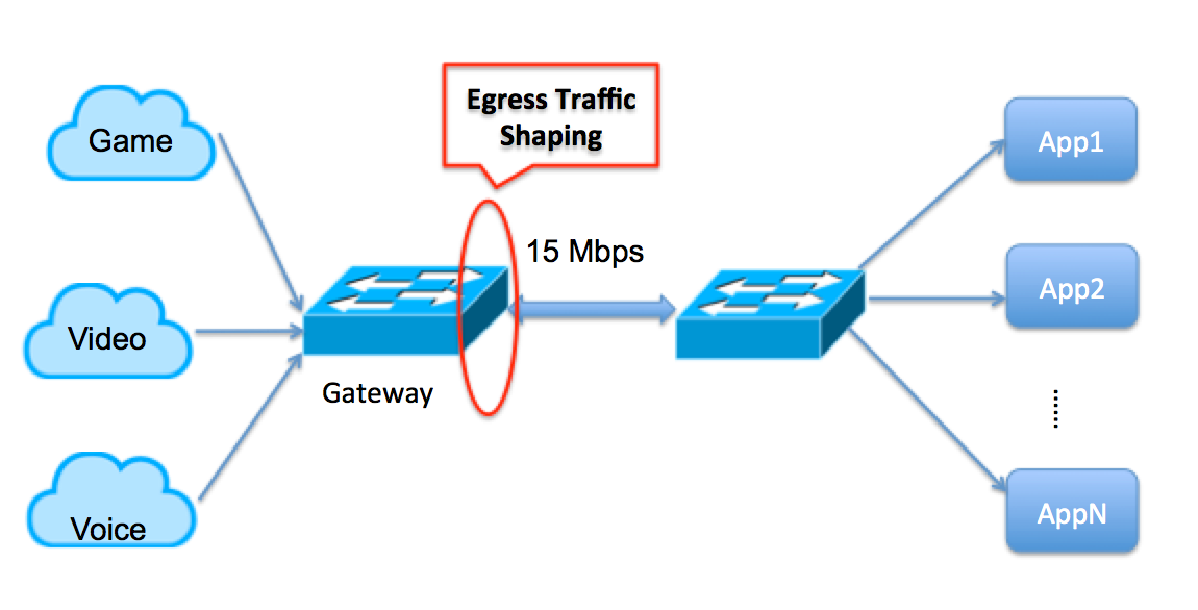
\includegraphics[width=0.5\textwidth]{exp_setup}
\caption{}
\label{fig:setup}
\end{figure}

During the experiments, hosts request different service, such as watching a video or making a VoIP call, depending on the experiment. 

We now show our system imporve the QoS of services in the face of competing traffic.
\subsubsection{Scenario 1}
In this scenario, one host is watching videos and the other host is downloading a file. And the priority of video is configured to be higher than file downloading. We generate traffic for the two services at the same time.

Figure illustrates the bitrates of the two services with our system, and Figure shows the bitrates of the two services withour our system. 

The results show that our system allows the system to quickly converge to a higher bitrate than it otherwise would without FlowQoS enabled. This prevents
bitrate oscillations and ensures the stability of the video player in terms of requested bitrates and video quality.
Thus, our system improves the quality of the adaptive streaming video by both reducing bitrate oscillation and achieving a higher overall bitrate.

\subsubsection{Scenario 2}
The setting of this scenarios is the same as last one. But we generate traffic for file downloading first, then generate traffic for video, then we stop traffic for vidoe to see how the file downloading rate change.

\subsubsection{Scenario 3}
We also evaluated our system in the context of VoIP application traffic. VoIP is sensitive to delay and variation in packet arrival times, so lower jitter is essential for good performance. We monitor the packet delay and jitter of the
VoIP application using ping and iperf to monitor the RTT and the packet arrival times throughout the experiment.




